% !TEX encoding = UTF-8
% !TEX TS-program = pdflatex
% !TEX root = ../tesi.tex

%**************************************************************
\chapter{Progetto di stage}
\label{cap:progetto-stage}

L'azienda \azienda{} ha da sempre mostrato interesse nell'inserimento all'interno del contesto aziendale di stagisti, studenti o altre figure professionali, anche per limitati periodi di tempo. Questa particolare propensione permette all'azienda sia di promuovere nuovi progetti o attività, che con il personale a disposizione non sarebbero percorribili per questioni di tempo, sia introdurre idee e tecnologie innovative per futuri prodotti o per quelli già sviluppati ed utilizzati da \azienda{}.\\ 

\section{Descrizione del progetto}
Negli ultimi anni \azienda{} si è interessata allo creazione e sviluppo di \gls{chatbot} per Facebook Messenger, dando la possibilità ai clienti di richiederne lo sviluppo di nuovi secondo le proprie specifiche, oppure di creare il proprio \gls{chatbot} autonomamente, senza alcuna conoscenza tecnica, attraverso dei template ottimizzati per i più comuni modelli di business. Questa nuova tecnologia è in rapida diffusione in svariati ambiti grazie alla sua facilità di sviluppo, esistono infatti molti tool che permettono di costruire il proprio \gls{chatbot} in pochi semplici passi.\\
Il progetto di stage si inserisce in questo ambito, in quanto l'azienda desiderava introdurre la possibilità per gli utenti di scrivere delle vere e proprie domande al \gls{chatbot}, senza dover utilizzare il menù o i pulsanti dei vari modelli che la piattaforma mette a disposizione.
\begin{figure}[h]
	\centering
	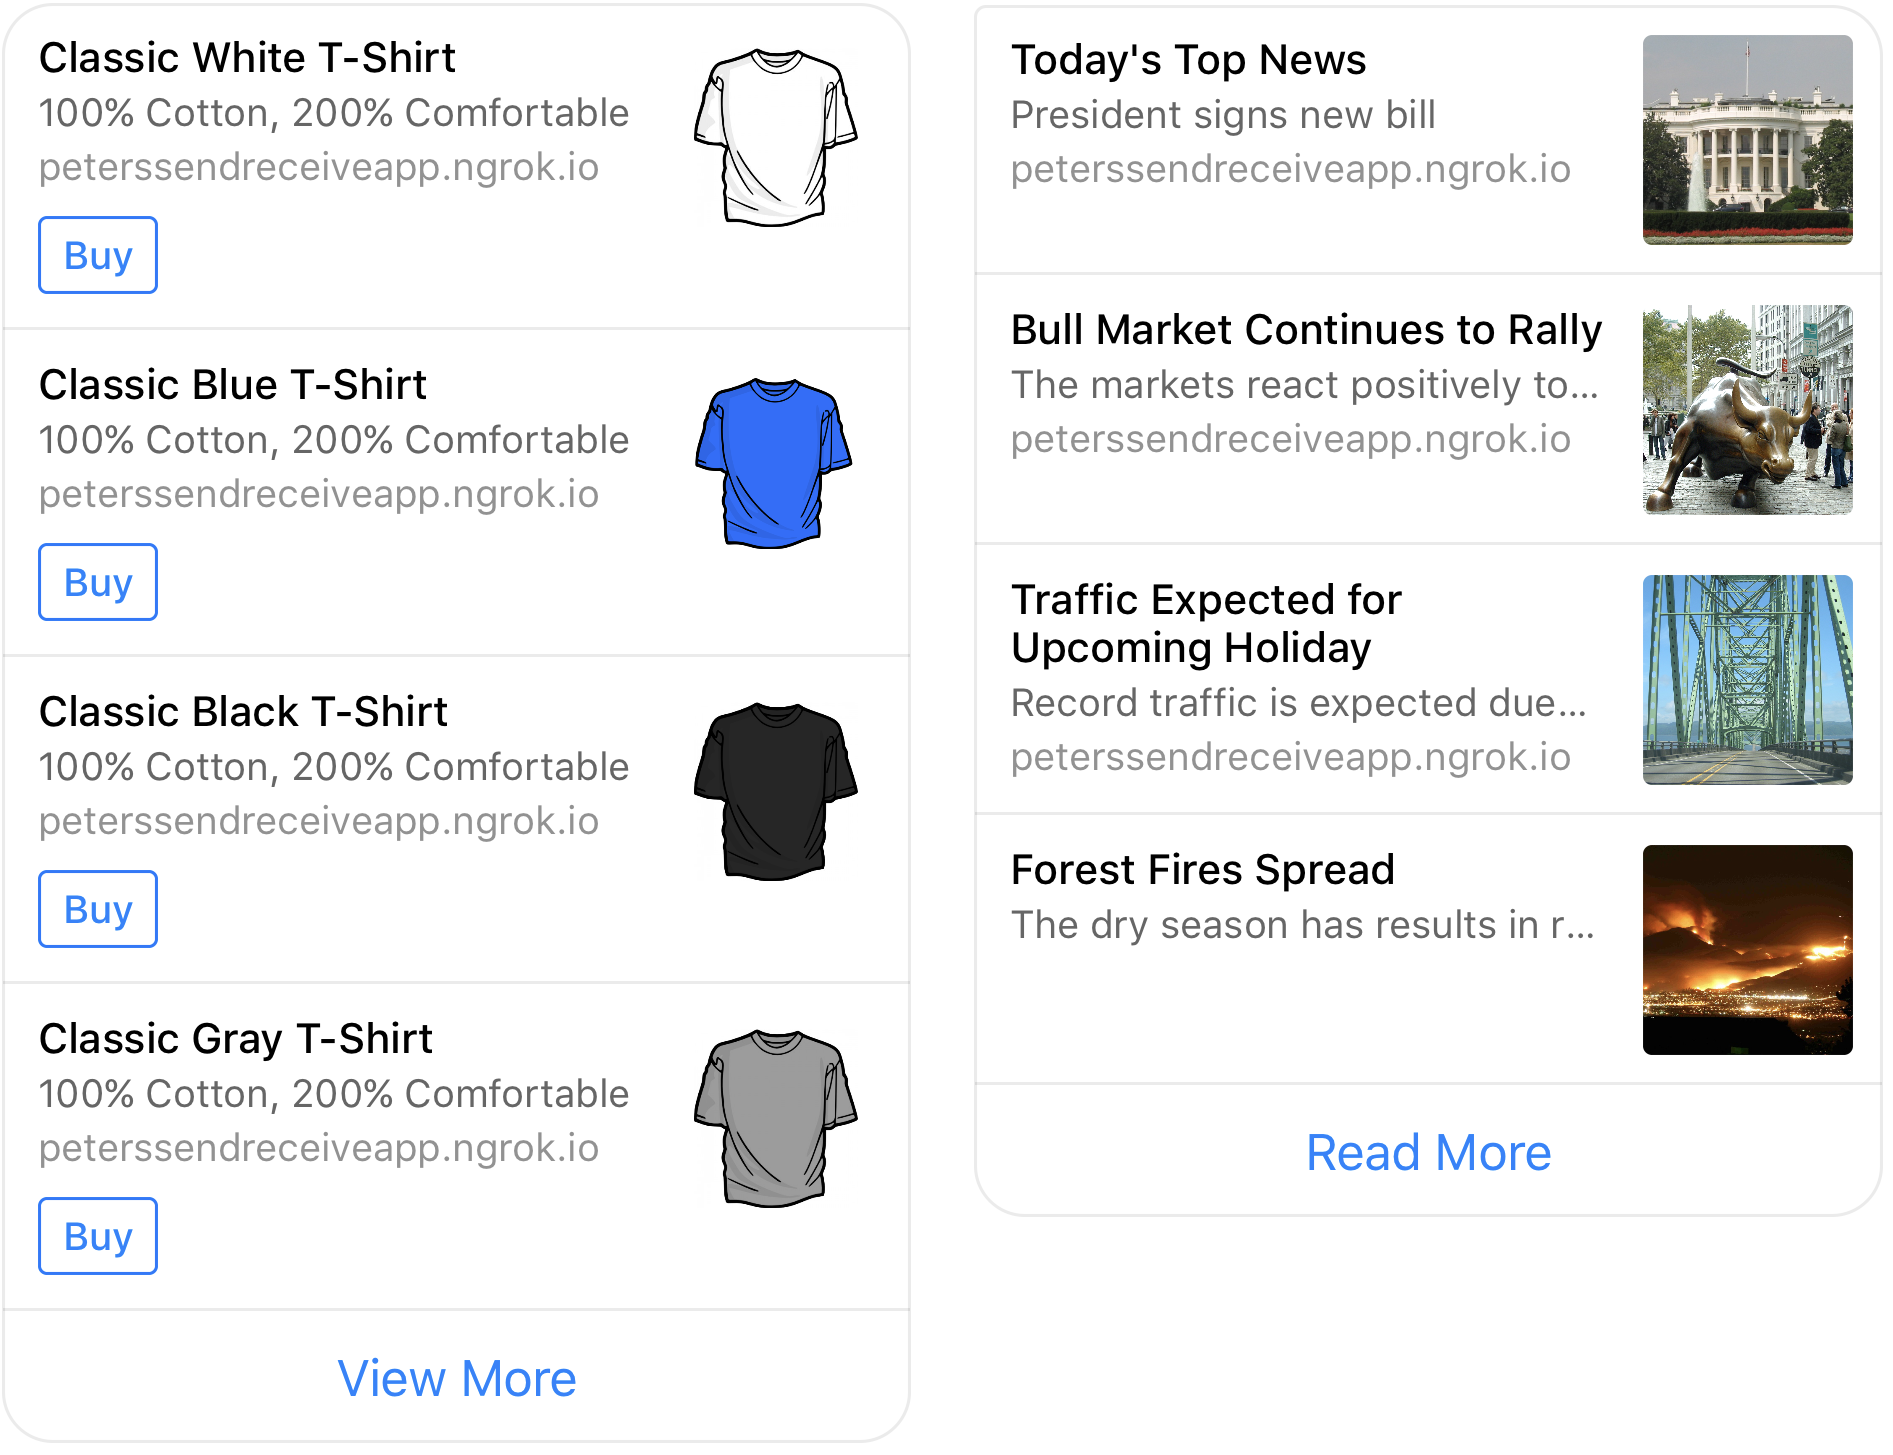
\includegraphics[scale=0.2]{../Immagini/modello_lista.png}
	\caption{Modello generico di carosello per Facebook Messenger}
\end{figure}
\newpage
Il compito assegnato allo stagista è stato quello di integrare questo meccanismo in due diversi \gls{chatbot} creati dall'azienda:
\begin{itemize}
	\item \textbf{gestore eventi}: è un applicativo creato da \azienda{} per essere utilizzato durante lo svolgimento di eventi della durata di uno o più giornate. Attraverso questo \gls{chatbot} l'utente può recuperare delle informazione riguardanti le conferenze in programma, le aule disponibili e le giornate dell'evento;
	\item \textbf{meteo Veneto bot}\footcite{meteo} questo \gls{chatbot} utilizza i dati di ARPA Veneto\footcite{arpav} per mostrare le previsioni del tempo del Veneto;
\end{itemize}
Il progetto si divideva quindi in tre parti:
\begin{itemize}
	\item analisi preliminare degli SDK delle principali piattaforme per il \gls{NLP} presenti sul mercato, in modo da valutarne pregi e difetti;
	\item creazione della logica per la gestione delle domande utente all'interno della piattaforma scelta;
	\item integrazione di questa nuova funzionalità nel software utilizzato da \azienda{} per la gestione dei \gls{chatbot}. 
\end{itemize}
Visto il bisogno di un periodo iniziale di studio, sia per capire le possibilità e i limiti degli strumenti da dover utilizzare nella trasformazione delle \gls{FAQ} in dati processabili, sia per apprenderne a pieno il funzionamento tramite la documentazione presente, \azienda{} ha ritenuto questo progetto idoneo ad uno studente universitario, il quale ha a disposizione circa 300 ore per formarsi su tutto ciò di cui vi è bisogno, e successivamente portare a termine il prodotto richiesto.

\section{Obiettivi dello stage}
\label{obiettivi}
Prima di iniziare il periodo di stage, sono stati discussi insieme al tutor aziendale i requisiti che il prodotto finale doveva soddisfare. Questi obiettivi sono stati raccolti in due categorie: obbligatori e desiderabili, a seconda dell'importanza della loro implementazione.

\subsection{Obiettivi obbligatori}
\begin{itemize}
	\item analisi del problema e studio delle possibili soluzioni già esistenti nel mercato;
	\item analisi e confronto delle piattaforme per il \gls{NLP};
	\item progettazione delle categorie di domande che la piattaforma deve gestire;
	\item sviluppo client di prova integrato tramite la piattaforma di \gls{NLP};
	\item sviluppo dell'integrazione della piattaforma con Facebook Messenger.
\end{itemize}

\subsection{Obiettivi desiderabili}
\begin{itemize}
	\item test e monitoraggio dell’applicativo tramite l’integrazione con 2 pagine Facebook reali.
\end{itemize}

\section{Principali problematiche}
Durante il periodo di stage, sono state incontrare diverse difficoltà, utili a migliorare la capacità di scelta e decisione dello stagista, ma anche la comunicazione e il lavoro all'interno di un team.

\subsection{Difficoltà di ambientazione}
Nei primi giorni in azienda l'ostacolo principale è stato l'inserimento in un team di lavoro affiatato e di esperienza, nonostante i suoi componenti siano stati molto disponibili e aperti a domande e chiarimenti. In particolare:
\begin{itemize}
	\item il \textbf{linguaggio tecnico/aziendale} non è stato da subito di facile apprendimento. In parte il problema sorgeva quando i brainstorming del team vertevano su tecnologie a me sconosciute, oppure su aspetti tecnici dei loro prodotti. Con il passare del tempo, attraverso l'utilizzo di un piccolo glossario individuale dove segnavo le spiegazioni dei termini a me non chiari, ho assimilato la maggior parte dei concetti, potendo così partecipare alle riunione del team in modo attivo e costruttivo;
	\item lavorare all'interno di un team non è un'attività semplice. Bisogna imparare a rispettare le scadenze nel rispetto dei colleghi e saper elaborare strategie nel caso in cui essi non siano riusciti a rispettare le proprie. Grazie all'esperienza che ho maturato sotto questo punto di vista, ho capito quanto sia importante pianificare con cura le attività e il tempo da destinare ad ognuna di esse.
\end{itemize}

\subsection{Difficoltà lavorative}
Durante lo svolgimento del mio progetto ho riscontrato queste difficoltà principali:
\begin{itemize}
	\item scelta del \textbf{miglior strumento per il \gls{NLP}}: il \gls{NLP} è un problema che è stato affrontato relativamente recentemente nel mondo dell'informatica. Le tecnologie che il mercato mette a disposizione sono limitate e spesso non soddisfacenti per gli obiettivi che mi sono stati richiesti. La ricerca di uno strumento idoneo non è stata facile, anche perchè l'azienda richiedeva non ci fossero costi per il suo utilizzo. Dopo una buona analisi del mercato, con la produzione di una relativa documentazione consegnata al tutor aziendale, è stato deciso di utilizzare Api.ai, servizio acquistato da Google nel 2016, che offre svariate funzionalità senza alcun costo, ma con delle sole limitazioni in termini di richieste giornaliere e mensili (una breve analisi dei principali strumenti di NLP è presente nella sezione???);
	\item \textbf{possibili richieste degli utenti}: il mio compito era quello di fornire una risposta tramite i \gls{chatbot} alle possibile domande di un utilizzatore. Se in primo momento questo non sembrava un \emph{task} troppo complicato, si è però trasformato in un problema non di semplice gestione, in quanto il dominio di richieste di un utente può essere vasto e molto vario. Per cercare di superare questo ostacolo, in accordo con il tutor e il team aziendale, si è deciso di limitare le categorie di domande a cui il \gls{chatbot} risponde, fornendo un messaggio adeguato in caso di una richiesta dell'utente non gestita. Sarà poi compito dell'azienda ampliare le funzionalità dei \gls{chatbot}, visto il poco tempo a mia disposizione, valutando le richieste fatte dagli utenti nell'apposita sezione di Api.ai;
	\item \textbf{gestione del sessionId}: nel JSON utilizzato per interrogare Api.ai tramite una richiesta PUSH, deve essere presente obbligatoriamente il campo sessionId, per identificare univocamente il mittente della richiesta. La gestione di questo campo è stata quindi di notevole importanza nel garantire ad ogni utente una corretta interazione con il \gls{chatbot}. Per assegnare ad ogni utente un sessionId univoco è stato deciso di creare un campo nella tabella degli utenti del database, dove memorizzare la stringa rappresentata dall'id dell'utente nel database e il timestamp del collegamento al bot, garantendo così l'unicità della stessa. In questo modo le domande fatte dall'utente al \gls{chatbot} saranno gestite come una conversazione, invece che una singola domanda senza una storia;
\end{itemize}

\section{Strumenti utilizzati}
\subsection{NetBeans}
NetBeans è un ambiente di sviluppo integrato multi-linguaggio, nato nel giugno 2000 e scritto interamente in Java, scelto dalla Oracle Corporation come IDE ufficiale da contrapporre al più diffuso Eclipse.
L'azienda non ha posto nessun vincolo sull'ambiente di sviluppo da adottare, così come vale per i propri dipendenti. Ho deciso di utilizzare NetBeans in quanto è molto intuitivo e di semplice utilizzo.\\
Inoltre offre una integrazione con \gls{Mercurial} per gestire \emph{push}, \emph{pull} e \emph{commit} senza utilizzare le righe di comando.
\begin{figure}[h]
	\centering
	
\includegraphics[scale=0.4]{../Immagini/netbeans.jpg}
	\caption{Logo di NetBeans}
\end{figure}
\subsection{Api.ai}
Api.ai è una società nata nell'ottobre del 2010 e acquisita da Google Inc. nel 2016. Api.ai è una piattaforma di conversazione
che permette interazioni sofisticate con il linguaggio naturale. All'interno del progetto è stata utilizzata per trasformare le domande degli utenti in dati processabili, dopo aver creato due agenti, uno per ciascun \gls{chatbot}, ed averli istruiti secondo le possibili \gls{FAQ} dei rispettivi ambiti di utilizzo.\\
Api.ai poteva essere integrato nel software aziendale in due diversi modi:
\begin{itemize}
	\item connesso direttamente al \gls{chatbot} di Facebook Messenger, grazie alla semplice integrazione prevista da Api.ai, estraendo le informazioni dal database aziendale tramite dei \emph{webhook}, anch'essi facilmente gestibili tramite la piattaforma di Api.ai;
	\item come strumento esterno al software aziendale, con il bisogno di interrogarlo tramite delle richieste POST HTTP solo in alcuni casi specifici, con le domande poste dall'utente.
\end{itemize} 
Dopo aver valutato entrambe le opzioni, ho scelto di intraprendere la seconda per due motivazioni:
\begin{itemize}
	\item utilizzando Api.ai come strumento esterno non è stato necessario introdurre dipendenze verso di esso nel codice, dando così la possibilità, se ci fosse bisogno in futuro, all'azienda di cambiare questa tecnologia con un'altra senza grossi problemi, cosa che sarebbe stata molto più difficile nell'altro caso;
	\item Api.ai mette a disposizione un SDK per Java molto utile, anche se non ben documentato. In ogni caso dopo aver capito il suo funzionamento è stato semplice sfruttarlo per interrogare Api.ai con poche righe di codice. 
\end{itemize}
\begin{figure}[h]
	\centering
	
\includegraphics[scale=0.2]{../Immagini/apiai.png}
	\caption{Logo di api.ai}
\end{figure}
\subsection{Hibernate}
Hibernate è una piattaforma open-source ad alto rendimento per lo sviluppo di applicazioni Java, che fornisce il servizio Object-relation mapping (ORM), ovvero si occupa della mappatura tra le classi Java e le relative tabelle di un database SQL.
Gestisce dunque il salvataggio degli oggetti di tali classi ed il reperimento dalle entità dal database, automatizzando le query necessarie e provvedendo alla reistanziazione dell’oggetto mappato sul database.
\begin{figure}[h]
	\centering
	
\includegraphics[scale=0.35]{../Immagini/Hibernate.png}
	\caption{Logo di Hibernate}
\end{figure}

\subsection{Database MySQL} 
L'azienda \azienda{} utilizza un database MySQL per la memorizzazione e gestione dei dati relativi ai progetti dei \gls{chatbot}. È il più diffuso database Open Source basato sul linguaggio SQL ed è di tipo relazionale, ovvero segue il principio che tutti i dati sono rappresentati come relazioni e manipolati con gli operatori dell’algebra relazionale o del calcolo relazionale.
Lo stagista è stato incaricato di capirne la struttura e come esso veniva gestito all'interno dell'applicativo, per poi utilizzarlo al meglio nello sviluppo del proprio prodotto.\\

\subsection{Strumenti aziendali}
Infine sono stati utilizzati alcuni degli strumenti consolidati nel contesto aziendale, come \emph{BitBucket} e \emph{Mercurial} per quanto riguarda il versionamento del codice, \emph{Slack} per le comunicazioni con gli altri dipendenti e il tutor ed \emph{Asana} per il tracciamento dei \emph{task} da svolgere (strumenti esposti nella sezione \ref{Teconologie}).

\section{Prodotto ottenuto}
Il prodotto che mi è stato richiesto di sviluppare consisteva nell'incremento delle funzionalità di due \gls{chatbot}, creati e gestiti da \azienda{}, per offrire agli utenti uno strumento che si avvicinasse il più possibile ad una chat normale con un essere umano.\\
Al mio arrivo in azienda questi due prodotti potevano essere utilizzati dagli utenti solamente attraverso l'interfaccia grafica che mettono a disposizione. In particolare, per i \gls{chatbot} di Facebook Messenger è possibile creare un menù, usufruibile in qualsiasi momento attraverso il pulsante rappresentato dalle 3 righe orizzontali, dove inserire dei comandi per mostrare determinate categorie di informazioni (ad esempio nel bot per le previsioni del tempo esiste il comando "Previsioni" che mostra il meteo per tutta la settimana, nella zona di interesse). Ci sono poi altri "caroselli" messi a disposizione dello sviluppatore per costruire le proprie risposte, spiegati ed illustrati nella documentazione di Facebook for Developers.\\

I risultati che sono riuscito ad ottenere nelle 300 ore di stage sono stati ritenuti molto soddisfacenti dall'azienda, e vengono illustrati attraverso degli esempi per i due diversi \gls{chatbot}.

\subsubsection{Meteo Veneto Bot}
Si tratta di un \gls{chatbot} innovativo che sfrutta i dati messi a disposizione da ARPA Veneto attraverso un file XML. I compito di questo  \gls{chatbot} è di dare delle informazioni all'utente sulle previsioni del tempo nella regione del Veneto, in particolare nella zona di interesse dell'utente che specifica all'inizio della conversazione inviando la propria posizione, o scrivendo il comune che desidera. Dopo aver premuto i pulsante "Previsioni", presente nel menù, si possono visualizzare i dettagli del meteo dei vari giorni della settimana, che mostrano temperature, precipitazione, venti ed ascoltare il bollettino.\\
Al termine del mio lavoro sono state introdotte nuove funzionalità che permettono all'utente di domandare:
\begin{itemize}
	\item il meteo per un determinato giorno in un comune preciso;
	\item se è prevista pioggia, neve, sole, nebbia per un determinato giorno in un comune preciso;
	\item di ascoltare il bollettino emesso da ARPA Veneto.
\end{itemize}

Di seguito vengono mostrati una serie di domande che è possibile fare al \gls{chatbot}, con le relative risposte.

\subsubsection{Gestore di eventi}
Si tratta di un template di \gls{chatbot} sviluppato da \azienda{} che viene  personalizzato ogni qualvolta un cliente ne richieda l'utilizzo, mantenendo in ogni caso delle funzionalità principali. Il suo compito è quello di mostrare delle informazioni riguardanti l'evento per il quale il \gls{chatbot} è stato personalizzato. In particolare si possono ottenere delle indicazioni sulle conferenze, come orario, durata, argomento, e sulle sale presenti.\\
Il mio compito in questo caso era di rendere queste funzionalità di immediato utilizzo attraverso delle domande da chiedere al bot. Adesso è possibile chiedere:
\begin{itemize}
	\item in \textbf{generale}:
	\begin{itemize}
		\item il programma dell'evento, specificando giorno ora e sala (non obbligatoriamente tutti e tre);
	\end{itemize}
	\item per le \textbf{conferenze}:
	\begin{itemize}
		\item la durata;
		\item l'orario di inizio e fine;
		\item in che sala si svolge;
	\end{itemize}
	\item per le \textbf{sale}:
	\begin{itemize}
		\item le indicazioni per trovarla;
		\item quale conferenza si svolge in un determinato giorno e orario;
		\item la conferenza successiva a quella in corso;
	\end{itemize}
\end{itemize}

Una volta posta una domanda al \gls{chatbot}, e ricevuta la relativa risposta, è stato anche implementato un sistema che permette all'utente di fare lo stesso tipo di domanda, come se stesse colloquiando con un essere umano. Ad esempio:

\begin{itemize}
	\item[-] Utente: "Che conferenza si svolge alle 12 in Lum250?"
	\item[-] Bot: "Analisi matematica"
	\item[-] Utente: "E in P140?"
	\item[-] Bot: "Programmazione 1".
\end{itemize}
Nella seconda risposta il sistema ha tenuto conto della prima domanda fatta dall'utente, cercando così la conferenza che sis volge alle 12 in P140. Questo meccanismo è stato implementato grazie ai \emph{context} di Api.ai.

